\section{Case study: Software System model}
\label{sec:case_study_software_system}

\subsection{Model Specification}

\hspace{1cm} The Software System model shown in Listing \ref{lst:software_system_specification} 
is the same model introduced in Chapter 1 to demonstrate OCL constraints (see 
Figure \ref{fig:class_diagram_software_system}). As a reminder, this model represents 
a simplified operating system that manages applications through their lifecycle. 
It consists of two main classes: \texttt{System} and \texttt{Application}, connected 
through an association. The \texttt{System} maintains three collections 
(\texttt{loadedApps}, \texttt{installedApps}, and \texttt{runningApps}) representing 
different application states, and provides four operations to manage applications: 
\texttt{load}, \texttt{install}, \texttt{run}, and \texttt{stop}.

The \texttt{freeMemory} attribute represents available disk space, which decreases 
when applications are loaded. The \texttt{load} operation acts as a download action, 
reducing available memory when an application is acquired. The \texttt{install} 
operation processes all loaded applications at once, moving them from 
\texttt{loadedApps} to \texttt{installedApps}. When an application is running, it 
exists in both the \texttt{installedApps} and \texttt{runningApps} sets simultaneously. 
The \texttt{SystemApplication} association facilitates navigation between system and 
applications in this simplified model.

Note that the numerous postconditions like \texttt{sameInstalledAndRunning}, 
\texttt{sameRunning}, \texttt{sameMemory}, \texttt{sameLoaded}, \texttt{sameInstalled}, 
and the \texttt{unchanged} constraints serve as helper constraints in the verification 
context: since the Model Validator assigns random values to attributes when exploring 
possible states, these constraints ensure that attributes unaffected by an operation 
remain consistent between snapshots.

This model serves as an ideal case study for temporal property verification as it 
involves operations with clear sequential dependencies and state transitions that 
cannot be adequately expressed using standard OCL. The complete specification, 
including all constraints and operation contracts necessary for our verification 
experiments, is provided in Appendix A. This appendix contains the full USE model 
specification that forms the foundation for our temporal property verification.
% This model serves as an ideal case study for temporal property verification as it 
% involves operations with clear sequential dependencies and state transitions that 
% cannot be adequately expressed using standard OCL. The full specification below 
% includes all constraints and operation contracts necessary for our verification 
% experiments.

% \begin{lstlisting}[
%     caption={Specification of the Software System model in USE environment.},
%     label={lst:software_system_specification}
% ]
% model SoftwareSystem
% -- Classes
% class System
% attributes
%     id : Integer
%     freeMemory : Integer init = 10
%     loadedApps : Set(Application) init = Set{}
%     installedApps : Set(Application) init = Set{}
%     runningApps : Set(Application) init = Set{}
% operations
%     load(app : Application)
%     begin
%         self.loadedApps := self.loadedApps->including(app);
%         self.freeMemory := self.freeMemory - app.size;
%     end
%     install()
%     begin
%         self.installedApps := self.installedApps->union(self.loadedApps);
%         self.loadedApps := self.loadedApps->reject(true)->excluding(null);
%     end
%     run(app : Application)
%     begin
%         self.runningApps := self.runningApps->including(app);
%     end
%     stop(app : Application)
%     begin
%         self.runningApps := self.runningApps->excluding(app);
%     end
% end
% class Application
% attributes
%     id : Integer
%     size : Integer
% end
% -- Associations
% association SystemApplication between
%     System[1] role system
%     Application[0..*] role apps
% end
% -- Invariants
% constraints
% context System
%     inv memoryConstraint: self.freeMemory >= 0
%     inv notLoadedAndInstalled: self.loadedApps->intersection(self.installedApps)->isEmpty()
%     inv sets: let appNumber: Integer = self.apps->size() in
%         (self.loadedApps->size() <= appNumber and
%         self.installedApps->size() <= appNumber and
%         self.runningApps->size() <= appNumber)
%     inv notContainsNull:
%         not self.loadedApps->includes(null) and
%         not self.installedApps->includes(null) and
%         not self.runningApps->includes(null)

% context Application
%     inv sizeConstraint: self.size > 0

% context System::load(app: Application)
%     pre notLoaded: not self.loadedApps->includes(app) and
%                     not self.installedApps->includes(app) and
%                     not self.runningApps->includes(app)
%     pre enoughMemory: self.freeMemory >= app.size
%     post loaded: self.loadedApps = self.loadedApps@pre->including(app)
%     post freeMemory: self.freeMemory = self.freeMemory@pre - app.size
%     post unchanged:
%         self.apps->forAll(app |
%             app.size = app.size@pre and
%             app.id = app.id@pre)
%     post sameInstalledAndRunning:
%         self.installedApps = self.installedApps@pre and
%         self.runningApps = self.runningApps@pre

% context System::install()
%     pre hasLoadedApps: self.loadedApps->notEmpty()
%     post installed: self.installedApps = self.installedApps@pre->union(self.loadedApps@pre)
%     post loadedAppsEmpty: self.loadedApps = self.loadedApps@pre->reject(true)->excluding(null)
%     post sameRunning: self.runningApps = self.runningApps@pre
%     post sameMemory: self.freeMemory = self.freeMemory@pre
%     post unchanged:
%         self.apps->forAll(app |
%             app.size = app.size@pre and
%             app.id = app.id@pre)

% context System::run(app : Application)
%     pre isInstalled: self.installedApps->includes(app)
%     pre notRunning: not self.runningApps->includes(app)
%     post running: self.runningApps = self.runningApps@pre->including(app)
%     post sameLoaded: self.loadedApps = self.loadedApps@pre
%     post sameInstalled: self.installedApps = self.installedApps@pre
%     post sameMemory: self.freeMemory = self.freeMemory@pre
%     post unchanged:
%         self.apps->forAll(app |
%             app.size = app.size@pre and
%             app.id = app.id@pre)

% context System::stop(app : Application)
%     pre isRunning: self.runningApps->includes(app)
%             and self.installedApps->includes(app)
%     post notRunning: self.runningApps = self.runningApps@pre->excluding(app)
%     post sameInstalled: self.installedApps = self.installedApps@pre
%     post sameLoaded: self.loadedApps = self.loadedApps@pre
%     post sameMemory: self.freeMemory = self.freeMemory@pre
%     post unchanged:
%         self.apps->forAll(app |
%             app.size = app.size@pre and
%             app.id = app.id@pre)
% \end{lstlisting}


\subsection{Temporal Property Verification}
% For each of the 4 properties:
%   1. Brief description of what the property verifies
%   2. TOCL+ specification
%   3. Generated OCL translation
%   4. Verification results

% The TOCL+ temporal properties for the Software System model were shown in Listing 
% \ref{lst:tocl+}. And Listing \ref{lst:ocl_translations} shows the OCL translations 
% for those TOCL+ properties. 

\hspace{1cm} To demonstrate our TOCL+ to OCL transformation approach, we verified four temporal 
properties from Chapter 2 against the Software System model: safety1 (applications 
must be loaded before being run), safety2 (applications must follow the 
load-install-run sequence), safety3 (applications are loaded at most once), and 
liveness (loaded applications will eventually be installed). Additionally, we 
formulated an alternative version of the liveness property using the 
\texttt{becomesTrue} event construct (Listing \ref{lst:liveness_becomesTrue}) to 
demonstrate this feature of our language. 

\begin{lstlisting}[
    style=toclstyle,
    caption={Liveness property using becomesTrue event.},
    label={lst:liveness_becomesTrue}
]
context Application
inv livenessBecomesTrue:
    self.system.loadedApps->includes(self) implies
    sometime becomesTrue(self.system.installedApps->includes(self))
\end{lstlisting}

Listing \ref{lst:ocl_translations} shows 
the OCL constraints generated by our transformation plugin for these properties. 
While the resulting OCL expressions are considerably more complex than their TOCL+ 
counterparts—involving extensive navigation through the filmstrip model—they 
correctly implement the required temporal semantics. This demonstrates how our 
approach enables temporal reasoning within standard OCL, shielding modelers 
from the underlying complexity.

\begin{lstlisting}[
    caption={OCL Translations for TOCL+ properties shown in listing \ref{lst:tocl+}.},
    label={lst:ocl_translations},
    captionpos=b
]
context System
inv safety1:
  self.runningApps->notEmpty() implies
  self.runningApps->forAll(app |
    (run_SystemOpC.allInstances()->exists(op | 
      op.succ() = self.snapshotSystem and 
      (Set{op.app.succApplication}->closure(p | p.succApplication)->includes(app) 
       or 
       Set{op.app.predApplication}->closure(p | p.predApplication)->includes(app))
    )) 
    implies
    (let CS:Snapshot = self.snapshotSystem in Set{CS.pred()}->closure(s | s.pred())->exists(s | (load_SystemOpC.allInstances()->exists(op | op.succ() = s and (Set{op.app.succApplication}->closure(p | p.succApplication)->includes(app) or Set{op.app.predApplication}->closure(p | p.predApplication)->includes(app))))))
  )

context System
inv safety2:
    self.runningApps->notEmpty() implies
    self.runningApps->forAll(app |
        (run_SystemOpC.allInstances()->exists(op | op.succ() = self.snapshotSystem and (Set{op.app.succApplication}->closure(p | p.succApplication)->includes(app) or Set{op.app.predApplication}->closure(p | p.predApplication)->includes(app)))) implies
        (let CS:Snapshot = self.snapshotSystem in let PS:Set(Snapshot) = Set{CS.pred()}->closure(s | s.pred())->excluding(null) in let AllPSQ:Set(Snapshot) = PS->select(s | (load_SystemOpC.allInstances()->exists(op | op.succ() = s and (Set{op.app.succApplication}->closure(p | p.succApplication)->includes(app) or Set{op.app.predApplication}->closure(p | p.predApplication)->includes(app))))) in let PSQ:Snapshot = AllPSQ->any(s | Set{s}->closure(s | s.pred())->includesAll(AllPSQ)) in let PSP:Set(Snapshot) = PS->select(s | install_SystemOpC.allInstances()->exists(op | op.succ() = s)) in if PSQ.isDefined() then (Set{PSQ}->closure(s | s.succ())->excluding(null)->intersection(PS)->exists(s | PSP->includes(s))) else false endif)
    )

context System
inv safety3:
    self.installedApps->notEmpty() implies
    self.installedApps->forAll(app |
        (let CS:Snapshot = self.snapshotSystem in Set{CS.pred()}->closure(s | s.pred())->exists(s | (load_SystemOpC.allInstances()->select(op | op.succ() = s and (Set{op.app.succApplication}->closure(p | p.succApplication)->includes(app) or Set{op.app.predApplication}->closure(p | p.predApplication)->includes(app)))->size() <= 1)))
    )

context System
inv liveness:
    self.loadedApps->notEmpty() implies
    self.loadedApps->forAll(app |
        (let CS:Snapshot = self.snapshotSystem in Set{CS}->closure(s | s.succ())->excluding(null)->exists(s | install_SystemOpC.allInstances()->exists(op | op.succ() = s)))
    )

context Application
inv livenessBecomesTrue:
    self.system.loadedApps->includes(self) implies
    (let CS:Snapshot = self.snapshotApplication in Set{CS}->closure(s | s.succ())->excluding(null)->exists(s | (let currentObject = s.application->any(o | o.id = self.id) in let previousObject = s.pred().application->any(o | o.id = self.id) in not (previousObject.system.installedApps->includes(previousObject)) and (currentObject.system.installedApps->includes(currentObject)))))
\end{lstlisting}


\subsection{Analysis of Results}

\hspace{1cm} Figure \ref{fig:object_diagram_case_study} shows a concrete scenario 
generated by the USE Model Validator when verifying our temporal properties. This 
scenario visualizes a complete application lifecycle through the software system, 
illustrating a sequence of operation calls: loading an application, installing it, 
running it, and finally stopping it. This execution path is particularly valuable 
as it exercises all four operations of our model in their expected sequence.

As shown in Figure \ref{fig:ocl_result_case_study}, all temporal properties are 
satisfied in this scenario. Each property verification confirms an important aspect 
of our system's behavior: safety1 verifies that the application was indeed loaded 
before being run; safety2 confirms the correct operational sequence was followed 
(load→install→run); safety3 validates that the application was loaded exactly once; 
and the liveness property confirms that after being loaded, the application was 
eventually installed.

These results demonstrate two important aspects of our approach. First, they validate 
the correctness of our transformation rules by confirming that the generated OCL 
constraints accurately encode the intended temporal semantics. Despite their 
complexity, the translated constraints correctly identify valid execution paths. 
Second, they show how our approach supports automated verification of complex 
temporal properties that would be impossible to express in standard OCL.

\begin{figure}[H]
    \centering
    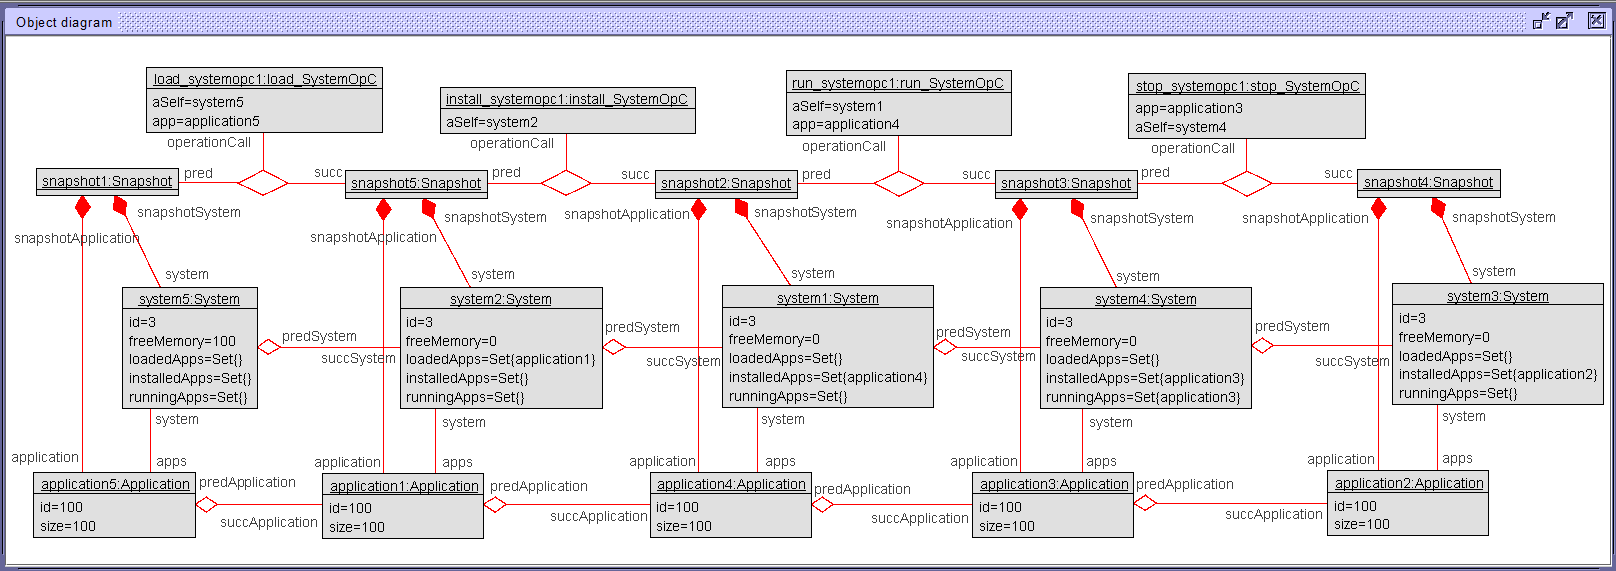
\includegraphics[width=1\textwidth]{figures/c3/CaseStudy_ObjectDiagram_2.png}
    \caption{A scenario generated by the USE Model Validator.}
    \label{fig:object_diagram_case_study}
\end{figure}

\begin{figure}[H]
    \centering
    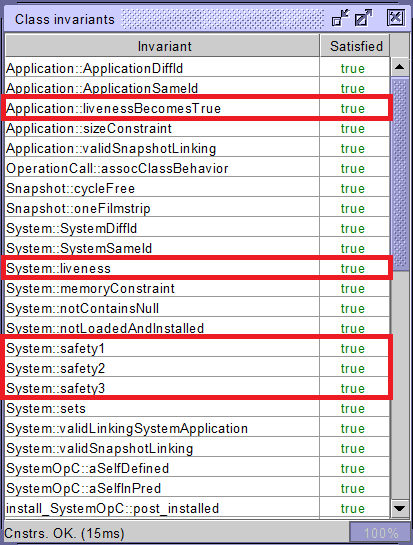
\includegraphics[width=0.4\textwidth]{figures/c3/OCL_result_full_1_edited.png}
    \caption{OCL result for generated scenario \ref{fig:object_diagram_case_study}.}
    \label{fig:ocl_result_case_study}
\end{figure}